\documentclass[12pt]{article}

\usepackage[a4paper]{geometry} %page size
\usepackage{parskip} %no paragraph indentation
\usepackage{fancyhdr} %fancy stuff in page header
\pagestyle{fancy} 

\usepackage[utf8]{inputenc} %encoding
\usepackage[danish]{babel} %danish letters

\usepackage{graphicx} %import pictures
\graphicspath{ {images/} }
\usepackage{listings} %make lists

\usepackage{amsmath, amssymb, amsfonts, amsthm, mathtools} %doing math
\usepackage{algorithmicx, algpseudocode} %doing pseudocode

\title{
  Title\
  \large Subtitle
}
\author{Asger Andersen}
\date{\today}

\fancyhead{}
\lhead{This is the title}
\rhead{Asger Andersen}

%End of preamble
%*******************************************************************************

\begin{document}

\section{Opgave 1: Kaniner og ræve}

Vi har modellen
\begin{align}
\begin{pmatrix}
K'(t) \\ 
R'(t)
\end{pmatrix} = f(K, R)
\end{align}
hvor 
\begin{align}
f(K,R) = \begin{pmatrix}
r_K K (1 - \alpha K - bR) \\ 
r_R R (cK - 1)
\end{pmatrix}
\end{align}
hvor $\alpha>0$, $b=0.05$, $c=0.005$ og $r_K = r_R = 2$.

\subsection{Delopgave a}

Hvis vi antager $R(t)=0$ for alle $t$, så forsimples modellen til
\begin{align}
f(K,R) = \begin{pmatrix}
r_K K (1 - \alpha K) \\ 
0
\end{pmatrix} = \begin{pmatrix}
r_K K \left(1 - \frac{K}{B}\right) \\ 
0
\end{pmatrix} 
\end{align}
hvor $B=1/\alpha$. Altså får vi en model, hvor der ingen ræve er, og hvor antallet af kaniner vokser logistisk med vækstraten $r_k=2$ og befolkningskapaciteten $B=1/\alpha$.

\subsection{Delopgave b}

\begin{enumerate}
\item Rævebestanden falder lige efter starttidspunktet.
\item Da er rævebestanden stigende og kaninbestanden faldende.
\item Der synes at være en ligevægt med omtrent 200 kaniner og omtrent 15 ræve.
\item Ligevægten ser lokalt stabil ud, da det den snurrende bevægelse ind mod ligevægten tyder på, at der i hvert er et åbent område omkring ligevægten, hvorindenfor enhver kombination af de to befolkningsstørrelser med tiden trækkes mod ligevægten som mod centrummet af en malstrøm.
\end{enumerate}

\subsection{Delopgave c}

\begin{enumerate}
\item Jeg udregner \begin{align}
f(K(0), R(0)) = \begin{pmatrix}
2\cdot 100 \left(1 - \frac{100}{1000} - \frac{5\cdot 10}{100} \right) \\ \\
2 \cdot 10 \left( \frac{5\cdot 100}{1000} - 1\right)
\end{pmatrix} = 
\begin{pmatrix}
80 \\
-10
\end{pmatrix}
\end{align}

Altså er $R'(0)=-10$, hvilket vil sige, at rævebestanden er faldende til starttidspunktet 0.
\item  Jeg udregner \begin{align}
f(300, 20) = \begin{pmatrix}
2\cdot 300 \left(1 - \frac{300}{1000} - \frac{5\cdot 20}{100} \right) \\ \\
2 \cdot 20 \left( \frac{5\cdot 300}{1000} - 1\right)
\end{pmatrix} = 
\begin{pmatrix}
-180 \\
20
\end{pmatrix}
\end{align}
Altså er kaninbestanden stigende og rævebestanden faldende, når der er 300 kaniner og 20 ræve.
\end{enumerate}

\subsection{Delopgave d \& e}

Jeg ønsker at bestemme, om modellen har ligevægte $(K^*, R^*)$, hvor $K^*, R^*>0$. Derfor vil forsøge at løse systemet
\begin{align}
f(K^*, R^*) = (0,0), \qquad K^*, R^*>0
\end{align}
hvilket vi kan skrive ud som
\begin{align}
\begin{pmatrix}
r_K K^* (1 - \alpha K^* - bR^*) \\ 
r_R R^* (cK^* - 1)
\end{pmatrix} =
\begin{pmatrix}
0 \\ 0
\end{pmatrix}, \qquad K^*, R^*>0
\end{align}
Da $r_K, r_R, K^*, R^*>0$, får vi det ækvivalente system
\begin{align}
\begin{pmatrix}
1 - \alpha K^* - bR^* \\ 
cK^* - 1
\end{pmatrix} =
\begin{pmatrix}
0 \\ 0
\end{pmatrix}, \qquad K^*, R^*>0
\end{align}
Den nederste ligning giver os, at
\begin{align}
K^* = \frac{1}{c}, \qquad K^* >0
\end{align}
Indsætter vi det i den æverste ligning, får vi
\begin{align}
1 - \alpha \frac{1}{c} - bR^*, \qquad R^*>0
\end{align}
hvilket er ækvivalent med
\begin{align}
R^* = \frac{1}{b}\left( 1 - \frac{\alpha}{c} \right), \qquad R^*>0
\end{align}
Da $a,b,c>0$, kan denne ligning kun være sand, hvis $\alpha<c=0.005$. Antager vi dette, får vi, at modellen har netop én ligevægt $(K^*, R^*)$, hvor $K^*, R^*>0$, nemlig
\begin{align}
\begin{pmatrix}
K^* \\ R^* 
\end{pmatrix} = \begin{pmatrix}
\frac{1}{c} \\ \\ 
\frac{1}{b}\left( 1 - \frac{\alpha}{c} \right)
\end{pmatrix} = \begin{pmatrix}
200 \\ \\
20\left( 1 - 200\alpha \right)
\end{pmatrix}
\end{align}

Jeg udregner funktionalmatricen for $f$ som
\begin{align}
Df(R,K) = \begin{bmatrix}
r_k(1 + bR -2\alpha K) & & -r_KbK \\ \\
r_RcR & & r_R(cK - 1)
\end{bmatrix}
\end{align}
Jeg evaluerer funktionalmatricen i ligevægten $(K^*, R^*)$:
\begin{align}
Df(R^*,K^*) =  \\ \\
\begin{bmatrix}
r_k\left(1 + b\left(\frac{1}{b}\left( 1 - \frac{\alpha}{c} \right) \right) -2\alpha\frac{1}{c} \right) & & -r_Kb\frac{1}{c} \\ \\
r_Rc\left(\frac{1}{b}\left( 1 - \frac{\alpha}{c} \right) \right) & & r_R\left(c\frac{1}{c} - 1\right)
\end{bmatrix} = \\ \\
\begin{bmatrix}
\frac{-r_Ka}{c} & & \frac{-r_Kb}{c} \\ \\
\frac{r_R}{c}( c- a ) & & 0
\end{bmatrix}
\end{align}
Jeg bestemmer det karakteristiske polynomien for funktionalmatricen evalueret i ligevægten:
\begin{align}
|Df(R^*,K^*) - \lambda E| = \\ 
\left(\frac{-r_K\alpha}{c} - \lambda \right)(-\lambda) + \frac{r_Kr_R(c-\alpha)}{c} = \\
\lambda^2 + \frac{r_K\alpha}{c}\lambda + \frac{r_Kr_R(c-\alpha)}{c}
\end{align}
Da vi har, at $r_K, r_R, \alpha, c>0$ og yderligere, at $\alpha<c$, er det karakteristiske altså på formen
\begin{align}
\lambda^2 + A\lambda + B, \qquad A,B >0
\end{align}
Rødderne i et sådant polynomien har negative realdele. Altså har funktionalmatricen evalueret i ligevægten kun egenværdier med negative realdele. Altså er ligevægten stabil per sætning 9 på side 150 i kursusbogen Differentialligninger.

Altså har vi nu alt i alt vist, at hvis $\alpha<c$, så har vores model netop én ligevægt $(K^*, R^*)$, hvor $K^*, R^*>0$, nemlig
\begin{align}
\begin{pmatrix}
K^* \\ R^* 
\end{pmatrix} = \begin{pmatrix}
200 \\ \\
20\left( 1 - 200\alpha \right)
\end{pmatrix}
\end{align}
og denne ligevægt er stabil. 

Sætter vi $\alpha = 0.001$, får vi altså den stabile ligevægt
\begin{align}
\begin{pmatrix}
K^* \\ R^* 
\end{pmatrix} = \begin{pmatrix}
200 \\ \\
20\left( 1 - \frac{200}{1000} \right)
\end{pmatrix} = \begin{pmatrix}
200 \\ \\
16
\end{pmatrix}
\end{align}
hvilket svarer til det, som det numeriske plot også syntes at vise.

\subsection{Delopgave f}

Lad mig nu vise, at hvis et polynomien har formen
\begin{align}
p(\lambda) = \lambda^2 + A\lambda + B, \qquad A,B >0
\end{align}
så har alle dets rødder negative realdele. 

Lad $\lambda = a + b i$ være en rod til $p$. Altså gælder
\begin{align}
\lambda^2 + A\lambda + B = 0, \qquad A,B >0
\end{align}
hvilket er ækvivalent med
\begin{align}
\lambda^2 + A\lambda = -B, \qquad A,B >0
\end{align}
hvilket, da $B>0$, medfører
\begin{align}
\lambda^2 + A\lambda < 0, \qquad A >0
\end{align}
Antag nu, at $b=0$, hvilket med andre ord vil sige, at $\lambda = a + b i$ er et reelt tal. Da har vi, at 
\begin{align}
a^2 + Aa < 0, \qquad A >0
\end{align}
Da $A, a^2>0$, har vi altså, at $a<0$, hvilket vil sige, at $\lambda$ har en negativ realdel.

Antag nu i stedet, at $b\neq 0$. Da har vi, at 
\begin{align}
(a + bi)^2 + A(a + bi) < 0, \qquad A >0
\end{align}
hvilket per udregning er ækvivalent med
\begin{align}
(a^2 - b^2 + Aa) + (b(A + 2a))i\ <\ 0, \qquad A >0
\end{align}
Da $(a^2 - b^2 + Aa) + (b(A + 2a))i\ <\ 0$, følger det, at $(a^2 - b^2 + Aa) + (b(A + 2a))i \in \mathbb{R}$, da udsagnet $\gamma < 0$ slet ikke er defineret, hvis $\gamma$ ikke er et reelt tal. Altså følger det, at
\begin{align}
b(A + 2a) = 0, \qquad A >0
\end{align}
Da vi antaget, at $b\neq 0$, er dette ækvivalent med
\begin{align}
2a = -A, \qquad A >0
\end{align}
Da $A>0$, har vi altså nu, at $a<0$. Altså har $\lambda$ en negativ realdel.

Jeg har nu alt i alt vist det ønskede.

\section{Opgave 2: }

\subsection{Delopgave a}

Vi har systemet 
\begin{align}
\begin{pmatrix}
V' \\ BC' 
\end{pmatrix} = f(V, BC)
\end{align}
hvor $f$ er defineret i opgavebeskrivelsen. Da opgavebeskrivelsen beder om at finde systemets ligevægt i ental, fortolker jeg det sådan, at det er givet, at der eksisterer netop ét punkt $(V^*,BC^*)\in \mathbb{R}$, så $V^*, BC^*>0$ (da ligevægten ellers er meningsløs fra et biologisk synspunkt) og så $f(V^*, BC^*) = (0,0)$. Altså er $(V^*, BC^*)$ det eneste strengt positive punkt i $\mathbb{R}^2$, så
\begin{align}
g(V^*, BC^*) = ||f(V^*, BC^*)|| = 0
\end{align}
Da normen af en vektor altid er større eller lig 0, så er $(V^*, BC^*)$ altså et globalt minimum for $g$ begrænset til domænet af strengt positive punkter i $\mathbb{R}^2$. Til forskel fra $f$ har $g$ et 1-dimensionelt output, og derfor kan $g$ minimeres ved hjælp af funktionen $nlm$ i R. Hermed finder jeg, at $(V^*, BC^*) = (0.43, 1.54)$.

Hvis vi betegner funktionalmatricen for $f$ med $Df$, kan vi let udregne, at 
\begin{align}
Df = \begin{bmatrix}
-(f_V + l_A) && 0 \\ \\
Df_{21} && Df_{22}
\end{bmatrix}
\end{align}
Altså er den transponerede funktionalmatrice en trekantsmatrice. En trekantsmatrice har sin diagonal som egenværdier. Da egenværdierne for en transponeret matrix er de samme som egenværdierne for matricen selv, får vi nu, at funktionalmatricen evalueret i ligevægten har egenværdierne
\begin{align}
\lambda_1 = -(f_V + l_A) = -0.3\\
\lambda_2 = Df_{21} = -\frac{f_C}{2}\left(\frac{BC^*}{V^*}\right)^2 \exp\left( \frac{BC^*}{V^*}\right) = -0.0037
\end{align}
Da begge egenværdier er skarpt negative, er ligevægten stabil.

\subsection{Delopgave b}

Her er to plots over den numeriske løsning med Eulers forbedrede metode ud fra de to forskellige startbetingelser:

\begin{center}
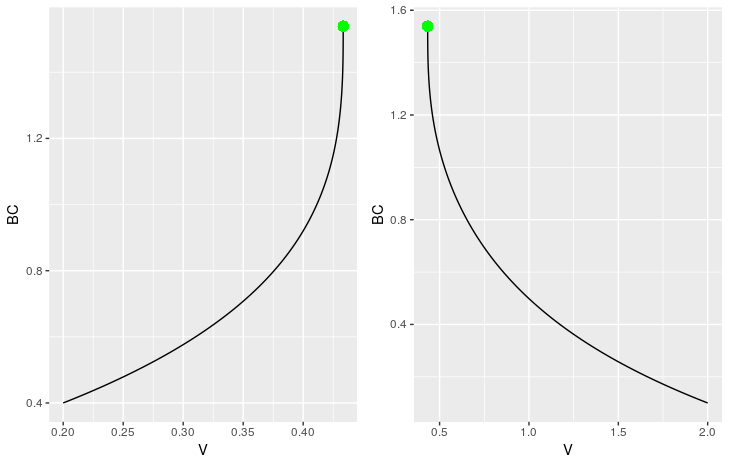
\includegraphics[scale=0.5]{q2p1.png}
\end{center}

Den grønne prik er ligevægten $(V^*, BC^*) = (0.43, 1.54)$. Jeg har simuleret udviklingen for $t=0,1,...,1500$.

\section{Opgave 3: Ulve, får og græs}

Vi har modellen 
\begin{align}
\begin{pmatrix}
G' \\ F' \\ U'
\end{pmatrix} = f(G, F, U)
\end{align}
hvor
\begin{align}
f(G, F, U) = \begin{pmatrix}
aG(1 - \alpha G - bF) \\
cF(dG - 1 - eU) \\
fU(\beta F - 1)
\end{pmatrix}
\end{align}
hvor $\alpha, \beta > 0$ og $a=2, b=0.001, c=0.1, d=0.01, e=0.2$ og $f=0.7$.

\subsection{Delopgave a}

Det fremgår af leddene $\beta F>0$ og $-eU<0$, at ulve spiser får. Hermed har vi nemlig, at ulvenes væksthastighed bør vokse med antallet af får, hvilket afspejles i leddet $\beta F>0$ i udtrykket for $U'(t)$. Ligeledes har vi, at fårenes væksthastighed bør falde med antallet af ulve, hvilket afspejles i leddet $-eU<0$ i udtrykket for $F'(t)$. 

Det fremgår, at ulve ikke spiser græs ved, at antallet af ulve $U$ ikke indgår i udtrykket for græssets væksthastighed $G'(t)$, og tilsvarende at mængden af græs $G$ ikke indgår i udtrykket for ulvebestandens væksthastighed $U'(t)$. Hermed udtrykker modellen, at mængden af ulve og græs ikke  påvirker hinanden direkte, men kun indirekte gennem mængden af får. 

\subsection{Delopgave b, c \& d}

For at bestemme modellens ligevægte skal vi løse systemet
\begin{align}
f(G^*, F^*, U^*) = \begin{pmatrix}
0 \\ 0 \\ 0
\end{pmatrix}
\end{align}

Fra 
\begin{align}
fU^*(\beta F^* - 1) = 0
\end{align}
får vi, at 
\begin{align}
U^* = 0
\end{align}
eller
\begin{align}
F^* = \frac{1}{\beta}
\end{align}

Antag først, at $U^*=0$. Indsætter vi dette resultat i 
\begin{align}
cF^*(dG^* - 1 - eU^*) = 0
\end{align}
får vi
\begin{align}
cF^*(dG^* - 1) = 0
\end{align}
hvilket giver, at 
\begin{align}
F^* = 0
\end{align}
eller 
\begin{align}
G^* = \frac{1}{d}
\end{align}

Antag først, at $F^*=0$. Indsætter vi dette resultat i 
\begin{align}
aG^*(1 - \alpha G^* - bF^*) = 0
\end{align}
får vi
\begin{align}
aG^*(1 - \alpha G^*) = 0
\end{align}
hvilket giver, at 
\begin{align}
G^* = 0
\end{align}
eller
\begin{align}
G^* = \frac{1}{\alpha}
\end{align}

Alt i alt har vi nu fundet ud, at systemet har de to ligevægte
\begin{align}
L_1 = \begin{pmatrix}
G_1^* \\ F^*_1 \\ U_1^*
\end{pmatrix} = \begin{pmatrix}
0 \\ 0 \\ 0
\end{pmatrix}, \qquad 
L_2 = \begin{pmatrix}
G_2^* \\ F^*_2 \\ U_2^*
\end{pmatrix} = \begin{pmatrix}
\frac{1}{\alpha} \\ 0 \\ 0
\end{pmatrix}
\end{align}

Antag nu fortsat, at $U^*=0$, men at $F^* \neq 0$. Da får vi fra vores resultater ovenfor, at
\begin{align}
G^* = \frac{1}{d}
\end{align}
Indsætter vi dette i
\begin{align}
aG^*(1 - \alpha G^* - bF^*) = 0
\end{align}
får vi
\begin{align}
\frac{a}{d}(1 - \frac{\alpha}{d} - bF^*) = 0
\end{align}
hvilket er ækvivalent med
\begin{align}
F^* = \frac{d-\alpha}{db}
\end{align}
Hermed har også fundet ligevægten
\begin{align}
L_3 = \begin{pmatrix}
G_3^* \\ F^*_3 \\ U_3^*
\end{pmatrix} = \begin{pmatrix}
\frac{1}{d} \\ \frac{d-\alpha}{db} \\ 0
\end{pmatrix}
\end{align}

Antag nu, at $U^*\neq 0$. Da får vi fra vores resultater ovenfor, at
\begin{align}
F^* = \frac{1}{\beta}
\end{align}
Indsætter vi dette i 
\begin{align}
aG^*(1 - \alpha G^* - bF^*) = 0
\end{align}
får vi 
\begin{align}
aG^*\left(1 - \alpha G^* - \frac{b}{\beta}\right) = 0
\end{align}
hvilket er ækvivalent med 
\begin{align}
-a\alpha (G^*)^2 + a \left( 1 - \frac{b}{\beta} \right) G^* = 0
\end{align}
Dette er en andengrads ligning med diskrimanten
\begin{align}
\text{dis} = \left(a \left( 1 - \frac{b}{\beta} \right) \right)^2 + 4a\alpha
\end{align}
Da $a, \alpha > 0$, har vi altså, at $d>0$, hvilket vil sige, at der er to ligevægte for $G$, nemlig
\begin{align}
G_4^* = \frac{a \left( 1 - \frac{b}{\beta} \right)  + \sqrt{\text{dis}}}{2a\alpha} 
\end{align}
og
\begin{align}
G_5^* = \frac{a \left( 1 - \frac{b}{\beta} \right) - \sqrt{\text{dis}}}{2a\alpha} 
\end{align}

Hvis vi indsætter dette i 
\begin{align}
cF^*(dG^* - 1 - eU^*) = 0
\end{align}
får vi nu også to ligevægte for $U^*$, nemlig
\begin{align}
U_4^* = \frac{dG_4^* - 1}{e} = 
\frac{d a \left( 1 - \frac{b}{\beta} \right)  + \sqrt{\text{dis}} - 2a\alpha}{2a\alpha e}
\end{align}
og 
\begin{align}
U_5^* = \frac{dG_5^* - 1}{e} = 
\frac{d a \left( 1 - \frac{b}{\beta} \right)  - \sqrt{\text{dis}} - 2a\alpha}{2a\alpha e}
\end{align}

Hermed har vi også fundet ligevægtene
\begin{align}
L_4 = \begin{pmatrix}
G_4^* \\ F^*_4 \\ U_4^*
\end{pmatrix} = \begin{pmatrix}
\frac{a \left( 1 - \frac{b}{\beta} \right)  + \sqrt{\text{dis}}}{2a\alpha}  \\ \\
\frac{1}{\beta} \\ \\
\frac{d a \left( 1 - \frac{b}{\beta} \right)  + \sqrt{\text{dis}} - 2a\alpha}{2a\alpha e}
\end{pmatrix}
\\
\\ 
L_5 = \begin{pmatrix}
G_5^* \\ F^*_5 \\ U_5^*
\end{pmatrix} = \begin{pmatrix}
\frac{a \left( 1 - \frac{b}{\beta} \right)  - \sqrt{\text{dis}}}{2a\alpha}  \\ \\
\frac{1}{\beta} \\ \\
\frac{d a \left( 1 - \frac{b}{\beta} \right)  - \sqrt{\text{dis}} - 2a\alpha}{2a\alpha e} 
\end{pmatrix}
\end{align}

Det var de generelle resultater. Lad os nu specialisere ved først at indsætte de fast givne  konstanter, samt sætte $\alpha=0.002$ og $\beta=0.005$. Hermed får vi disse ligevægte:
\begin{center}
% latex table generated in R 3.4.4 by xtable 1.8-2 package
% Mon May 14 00:46:43 2018
\begin{table}[ht]
\centering
\begin{tabular}{rrrr}
  \hline
 & G & F & U \\ 
  \hline
L1 & 0.00 & 0.00 & 0.00 \\ 
  L2 & 500.00 & 0.00 & 0.00 \\ 
  L3 & 100.00 & 800.00 & 0.00 \\ 
  L4 & 400.62 & 200.00 & 15.03 \\ 
  L5 & -0.62 & 200.00 & -5.03 \\ 
   \hline
\end{tabular}
\end{table}

\end{center}
Vi ser, at der er netop én strengt positiv ligevægt, nemlig $L_4$. Der er altså netop én ligevægt, hvor alle 3 arter overlever. I den ligevægt har vi 400 græs (hvad end det vil sige), 200 får og 15 ulve. Dog ved vi ikke noget om, hvilke startbetingelser, der fører til denne ligevægt frem for nogle af de andre.

Hvis vi sætter $\alpha=0.002$ og $\beta=0.0008$, får vi disse ligevægte
\begin{center}
% latex table generated in R 3.4.4 by xtable 1.8-2 package
% Mon May 14 00:46:44 2018
\begin{table}[ht]
\centering
\begin{tabular}{rrrr}
  \hline
 & G & F & U \\ 
  \hline
L1 & 0.00 & 0.00 & 0.00 \\ 
  L2 & 500.00 & 0.00 & 0.00 \\ 
  L3 & 100.00 & 800.00 & 0.00 \\ 
  L4 & 1.97 & 1250.00 & -4.90 \\ 
  L5 & -126.97 & 1250.00 & -11.35 \\ 
   \hline
\end{tabular}
\end{table}

\end{center}
Vi ser, at vi ikke længere har nogen strengt positiv ligevægt. Der er altså ikke nogle startbetingelser, der fører til en langsigtet udvikling, hvor alle 3 arter overlever. I denne verden vil ulvene altid uddø på sigt. Der findes dog en ligevægt, hvor både græsset og fårene overlever, nemlig $L_3$, hvor der er 100 græs og 800 får.

I forhold til før er det, der er ændret, at $\beta$ er blevet lavere, og det har altså gjort, at ulvene altid vil uddø på sigt. Ser vi på modellen, udtrykker $\beta$ netop i hvor høj grad flere får øger ulvenes væksthastighed. Sætter vi $\beta$ ned, formindskes ulvenes væksthastighed per får, og det giver umiddelbart mening, at dette forværre ulvenes mulighed for at overleve på lang sigt.

Hvis vi sætter $\alpha=0.02$ og $\beta=0.0008$, får vi disse ligevægte
\begin{center}
% latex table generated in R 3.4.4 by xtable 1.8-2 package
% Mon May 14 00:46:44 2018
\begin{table}[ht]
\centering
\begin{tabular}{rrrr}
  \hline
 & G & F & U \\ 
  \hline
L1 & 0.00 & 0.00 & 0.00 \\ 
  L2 & 50.00 & 0.00 & 0.00 \\ 
  L3 & 100.00 & -1000.00 & 0.00 \\ 
  L4 & 1.75 & 1250.00 & -4.91 \\ 
  L5 & -14.25 & 1250.00 & -5.71 \\ 
   \hline
\end{tabular}
\end{table}

\end{center}
Vi ser, at vi ikke længere har nogen strengt positiv ligevægt og heller ikke nogen ligevægt, hvor fårene overlever på lang sigt. I denne verden er græsset den eneste art, der har mulighed for at forblive i live i al fremtid. Interessant nok er forskellen på denne situation og situationen før, at vi har sat $\alpha$ op. Ser vi på modellen, udtrykker $\alpha$ i hvor høj grad græsset hæmmer sin egen vækst. At græsset hæmmer sin vækst mere får altså tilsyneladende fårene til at uddø på lang sigt, hvorefter græsset er den eneste art, der er tilbage. Dette har at gøre med, at fårene jo lever af græs, og derfor vil forskellen mellem $d$ (hvor meget græsset øger fårenes vækst) og $\alpha$ (hvor meget græsset hæmmer sin egen vækst) afgøre, om fårene kan overleve på lang sigt. Hvis græsset hæmmer sin vækst mere end det fremmer fårenes vækst (hvis $\alpha>d$), så vil fårene ifølge vores model uddø på lang sigt.

Nu mangler jeg bare at afgøre, om den strengt positive ligevægt i tilfældet $\alpha=0.002$ og $\beta=0.005$ er stabil eller ej. Her er funktionalmatricen for $f$
\begin{align}
Df = \begin{bmatrix}
a(1-2\alpha G - b F) && -abG && 0 \\ \\
cdF && c(dG-1-eU) && -ceF \\ \\ 
0 && f\beta U && f(\beta F - 1)
\end{bmatrix}
\end{align}
Jeg bruger R til at evaluere denne matrice i ligevægten $L_4$ for $\alpha=0.002$ og $\beta=0.005$, hvorefter jeg finder dens egenværdier. Hermed får jeg
\begin{align}
\lambda_1 = -1.51, \quad \lambda_2 = -0.05 + 0.47i, \quad \lambda_3 = -0.05 - 0.47i
\end{align}
Da alle disse tre egenværdier har negative realdele, er ligevægten stabil.

\end{document}